\documentclass{article}

%\documentclass[border=5]{standalone}

\usepackage{tikz}
%\usepackage{xcolor}
\usetikzlibrary{arrows,shapes,snakes,automata,backgrounds,petri, decorations.text,positioning, calc}

\begin{document}
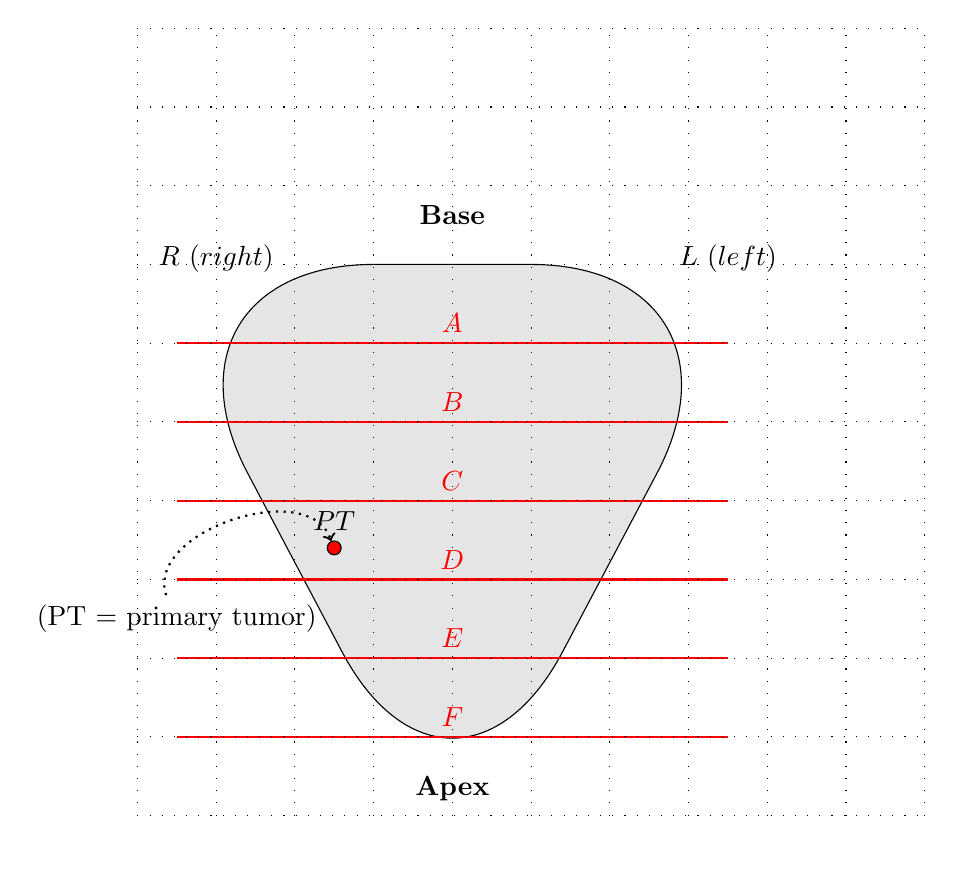
\begin{tikzpicture}%[scale=2]
  \draw [rounded corners=30mm,fill=gray!20] (0,7)--(8,7)--(4.0,-0.57)--cycle;

  \draw[thick, red] (  0.5,6)  -- node [above ] {\normalsize{$A$}} (7.5,6);
  \draw[thick, red] (  0.5,5)  -- node [above] {\normalsize{$B$}} (7.5,5);
  \draw[thick, red] (  0.5,4)  -- node [above] {\normalsize{$C$}} (7.5,4);
  \draw[thick, red] (  0.5,3)  -- node [above] {\normalsize{$D$}} (7.5,3);
  \draw[thick, red] (  0.5,2)  -- node [above] {\normalsize{$E$}} (7.5,2);
  \draw[thick, red] (  0.5,1)  -- node [above] {\normalsize{$F$}} (7.5,1);
  %\draw[thick, red] (  0.5,0)  -- node [above] {\normalsize{$G$}} (7.5,0);
  
  %label={[label distance=2mm]
  \node [circle,draw=black,fill=red,inner sep=0pt,minimum size=5pt,label={[label distance=0mm] {\normalsize{$PT$}}} ] (PT1) at (2.5,3.4) {};
  
  %%% fix me !!!
  %\node (box1) at  (0.5,2.5) [align=left] {\normalsize podejrzana pozycja guza\\\normalsize(PT = primary tumor)} ;
  
    \node (box1) at  (0.5,2.5) [align=left] {\normalsize (PT = primary tumor)} ;
  \draw[thick, dotted, ->]
  (box1) [bend left=90]  to  (PT1);



  \node [label=below:{\normalsize{$R\ (right) $}} ] (R) at (1.0,7.5) {};
  \node [label=below:{\normalsize{$L\ (left) $}} ] (L) at (7.5,7.5) {};
  \node [label=below:{\normalsize \bf Base} ] (base) at (4.0,8.0) {};
  \node [label=below:{\normalsize \bf Apex} ] (apex) at (4.0,0.75) {};

 

  % \node  (G) at (5,3.5) { G  } ;

  \draw[loosely  dotted] (0,0) grid (10,10);
\end{tikzpicture}
\end{document}
